\chapter{Introduction}

\section{Overview}
This book is about synchronic metathesis.
One well known case of synchronic metathesis comes
from Rotuman, in which many words have two forms,
such as \it{pu\tbr{re}} {\tl} \it{pu\tbr{er}} `rule, decide'
(\citealp[14]{ch40}, discussed in more detail in \srf{sec:Rot}).
In this book I present new data from Amarasi,
a language which also has synchronic metathesis.
Observe the natural textual data in \qf{ex:130902-1, 1.43 ch:Intr} below.

\begin{exe}
	\ex{Going to a party: \txrf{130902-1, 1.43}{\emb{130902-1-01-43.mp3}{\spk{}}{\apl}}}\label{ex:130902-1, 1.43 ch:Intr}
	\begin{xlist}
		\ex{\gll	oras hai m-nao =te, \\
							time {\hai} {\m}-go ={\te}\\
				\glt	`While we were going,' \txrf{}}
		\ex{\gll	naiʔ Owen ina ʔpiurʔ=ee n-mo\tbr{uf}, n-mo\tbr{fu} =ma na-mneuk.\\
							{\naiq} Owen {\iin} cloth={\ee} {\n}-fall {\n}-fall =and {\na}-lose\\
				\glt	`Owen's handkerchief fell, it fell and was lost.'}
	\end{xlist}
\end{exe}

The metathesis of Amarasi \ve{mofu} {\tl} \ve{mouf} `fall'
in \qf{ex:130902-1, 1.43 ch:Intr} is formally almost identical to Rotuman
metathesis in examples such as \it{pure} {\tl} \it{puer} `rule, decide'.
In each case the final CV sequence of a CVCV stem metathesises to VC,
as illustrated in \qf{as:Metathesis} below with
the architecture of Autosegmental Phonology \citep{go76}.

\begin{multicols}{3}
	\begin{exe}
		\ex{\begin{xlist}
			\exa{\xy
				<0em,2.5cm>*\as{\x}="x1",<1em,2.5cm>*\as{\x}="x2",<2em,2.5cm>*\as{\x}="x3",<3em,2.5cm>*\as{\x}="x4",,
				<0em,1.5cm>*\as{\hp{\sub{1}}C\sub{1}}="C1",<1em,1.5cm>*\as{\hp{\sub{2}}V\sub{2}}="V1",
				<2em,1.5cm>*\as{\hp{\sub{3}}C\sub{3}}="C2",<3em,1.5cm>*\as{\hp{\sub{4}}V\sub{4}}="V2",
				<0em,0.5cm>*\as{p}="c1",<1em,0.5cm>*\as{u}="v1",<2em,0.5cm>*\as{r}="c2",<3em,0.5cm>*\as{e}="v2",
				<0em,0cm>*\as{m}="c1a",<1em,0cm>*\as{o}="v1a",<2em,0cm>*\as{f}="c2a",<3em,0cm>*\as{u}="v2a",
				"C1"+U;"x1"+D**\dir{-};"V1"+U;"x2"+D**\dir{-};"C2"+U;"x3"+D**\dir{-};"V2"+U;"x4"+D**\dir{-};
				"c1"+U;"C1"+D**\dir{-};"v1"+U;"V1"+D**\dir{-};"c2"+U;"C2"+D**\dir{-};"v2"+U;"V2"+D**\dir{-};
			\endxy}
			\exa{\xy
				<0em,2.5cm>*\as{\x}="x1",<1em,2.5cm>*\as{\x}="x2",<2em,2.5cm>*\as{\x}="x3",<3em,2.5cm>*\as{\x}="x4",,
				<0em,1.5cm>*\as{\hp{\sub{1}}C\sub{1}}="C1",<1em,1.5cm>*\as{\hp{\sub{2}}V\sub{2}}="V1",
				<2em,1.5cm>*\as{\hp{\sub{3}}C\sub{3}}="C2",<3em,1.5cm>*\as{\hp{\sub{4}}V\sub{4}}="V2",
				<0em,0.5cm>*\as{p}="c1",<1em,0.5cm>*\as{u}="v1",<2em,0.5cm>*\as{r}="c2",<3em,0.5cm>*\as{e}="v2",
				<0em,0cm>*\as{m}="c1a",<1em,0cm>*\as{o}="v1a",<2em,0cm>*\as{f}="c2a",<3em,0cm>*\as{u}="v2a",
				"C1"+U;"x1"+D**\dir{-};"V1"+U;"x2"+D**\dir{-};"C2"+U;"x4"+D**\dir{.};"V2"+U;"x3"+D**\dir{.};
				"c1"+U;"C1"+D**\dir{-};"v1"+U;"V1"+D**\dir{-};"c2"+U;"C2"+D**\dir{-};"v2"+U;"V2"+D**\dir{-};
			\endxy}
			\exa{\xy
				<0em,2.5cm>*\as{\x}="x1",<1em,2.5cm>*\as{\x}="x2",<2em,2.5cm>*\as{\x}="x3",<3em,2.5cm>*\as{\x}="x4",,
				<0em,1.5cm>*\as{\hp{\sub{1}}C\sub{1}}="C1",<1em,1.5cm>*\as{\hp{\sub{2}}V\sub{2}}="V1",
				<2em,1.5cm>*\as{\hp{\sub{4}}V\sub{4}}="C2",<3em,1.5cm>*\as{\hp{\sub{3}}C\sub{3}}="V2",
				<0em,0.5cm>*\as{p}="c1",<1em,0.5cm>*\as{u}="v1",<2em,0.5cm>*\as{e}="c2",<3em,0.5cm>*\as{r}="v2",
				<0em,0cm>*\as{m}="c1a",<1em,0cm>*\as{o}="v1a",<2em,0cm>*\as{u}="c2a",<3em,0cm>*\as{f}="v2a",
				"C1"+U;"x1"+D**\dir{-};"V1"+U;"x2"+D**\dir{-};"C2"+U;"x3"+D**\dir{-};"V2"+U;"x4"+D**\dir{-};
				"c1"+U;"C1"+D**\dir{-};"v1"+U;"V1"+D**\dir{-};"c2"+U;"C2"+D**\dir{-};"v2"+U;"V2"+D**\dir{-};
			\endxy}		
		\end{xlist}}\label{as:Metathesis}
	\end{exe}
\end{multicols}

Synchronic metathesis in Amarasi is phonologically very similar
to previously described cases in other languages.
Furthermore, in certain environments the phonology alone
determines whether the metathesised or unmetathesised
form of a word will appear in Amarasi.
However, phonology alone cannot predict that reversal of the position of the
metathesised and unmetathesised words in \qf{ex:130902-1, 1.43 ch:Intr}
produces a sentence judged ungrammatical by native speakers,
as shown in \qf{ex:el. 22/02/16 p.19}.

\begin{exe}
	\ex[*]{\gll	naiʔ Owen ina ʔpiurʔ=ee n-mo\tbr{fu}, n-mo\tbr{uf} =ma na-mneuk.\\
						{\naiq} Owen {\iin} cloth={\ee} {\n}-fall {\n}-fall =and {\na}-lose\\
			\glt	`(Owen's handkerchief fell, it fell and was lost.)' \txrf{elicit. 22/02/16 p.19}
			}\label{ex:el. 22/02/16 p.19}
\end{exe}

The forms of synchronic metathesis in several languages have been well described.
This has lead to much useful discussion about the kinds
of phonological models which best handle metathesis,
as found in works including
\cite{be87,huen95,hu98,huse04,hu04}, and \cite{he04}, among others.

Despite this interest in the form of synchronic metathesis,
there has been relatively little attention given to
the functions of synchronic metathesis
and the different environments in which an unmetathesised
or metathesised form of a word is used.
This work partially redresses this imbalance.
I provide a detailed analysis of the functions and
environments of synchronic metathesis in Amarasi.
This includes one instance of phonologically conditioned metathesis
and two different morphological uses of metathesis,
neither of which can be reduced to a phonologically conditioned process.

I begin in Chapter \ref{ch:SynchMet} with a discussion
of processes of synchronic metathesis in languages of the world.
The focus in this chapter is on languages spoken in the same region
as Amarasi, particularly languages with morphological metathesis.
There are many similarities in both the form and use of metathesis in these languages.
Chapter \ref{ch:SynchMet} allows me to position the Amarasi
data within its geographic and typological context.

After a discussion of Amarasi phonology and phonotactics
in Chapter \ref{ch:AmaPho}, in Chapter \ref{ch:StrMetAma}
I provide a detailed investigation of the form of metathesis in Amarasi.
Depending on the phonotactic structure of the stem to which it applies,
metathesis is associated with a bewildering
array of disparate phonological processes including
vowel deletion, consonant deletion, consonant insertion,
and multiple kinds of vowel assimilation.
All these phonological processes
can be derived from a single process of metathesis and
one associated morphemically conditioned process
by proposing that Amarasi has an obligatory
CVCVC foot in which C-slots can be empty.

The structure of the words \ve{fatu} `stone', \ve{kaut} `papaya' and \ve{ai} `fire'
under this analysis are given in \qf{as:fatu/kaut/ai ch:Int} below.
Evidence independent of metathesis for empty C-slots in Amarasi 
is presented in (\srf{sec:EmpCSlo}).
Such evidence consists of five language-internal
phenomena as well as comparative data.

\begin{multicols}{3}
	\begin{exe}
		\ex{\begin{xlist}
			\exa{\xy
				<0cm,1cm>*\as{C}="C1",<1em,1cm>*\as{V}="V1",<2em,1cm>*\as{C}="C2",<3em,1cm>*\as{V}="V2",<4em,1cm>*\as{C}="C3",
				<0em,0cm>*\as{f}="c1",<1em,0cm>*\as{a}="v1",<2em,0cm>*\as{t}="c2",<3em,0cm>*\as{u}="v2",
				"c1"+U;"C1"+D**\dir{-};"c2"+U;"C2"+D**\dir{-};"v1"+U;"V1"+D**\dir{-};"v2"+U;"V2"+D**\dir{-};
			\endxy}
			\exa{\xy
				<0em,1cm>*\as{C}="C1",<1em,1cm>*\as{V}="V1",<2em,1cm>*\as{C}="C2",<3em,1cm>*\as{V}="V2",<4em,1cm>*\as{C}="C3",
				<0em,0cm>*\as{k}="c1",<1em,0cm>*\as{a}="v1",<3em,0cm>*\as{u}="v2",<4em,0cm>*\as{t}="c3",
				"c1"+U;"C1"+D**\dir{-};"c3"+U;"C3"+D**\dir{-};"v1"+U;"V1"+D**\dir{-};"v2"+U;"V2"+D**\dir{-};
			\endxy}
			\exa{\xy
				<0em,1cm>*\as{C}="C1",<1em,1cm>*\as{V}="V1",<2em,1cm>*\as{C}="C2",<3em,1cm>*\as{V}="V2",<4em,1cm>*\as{C}="C3",
				<1em,0cm>*\as{a}="v1",<3em,0cm>*\as{i}="v2",
				"v1"+U;"V1"+D**\dir{-};"v2"+U;"V2"+D**\dir{-};
			\endxy}
		\end{xlist}}\label{as:fatu/kaut/ai ch:Int}
	\end{exe}
\end{multicols}

The presence of phonological processes in addition to metathesis
leads me to label forms corresponding to unmetathesised forms as \emph{U\=/forms}
and those corresponding to metathesised forms as \emph{M\=/forms}.\footnote{
		The terms U\=/form and M\=/form can be taken as abbreviations for the form
		where \emph{U} stands for \emph{unmetathesised} and \emph{M} for \emph{metathesised}.
		They can also be taken as abbreviations for the functions of these forms,
		as in the syntax M\=/forms mark \emph{\tbf{m}odification}
		and in the discourse U\=/forms mark \emph{\tbf{u}nresolved} events or situations.
		The \emph{U} in U\=/form can also be an abbreviation for
		the morphologically \emph{\tbf{u}nderlying} form.}

In Chapter \ref{ch:PhoMet} I analyse phonologically conditioned metathesis in Amarasi.
Before vowel-initial enclitics, metathesis occurs
to clearly mark a phonological boundary between
a clitic host and vowel-initial enclitic.
The final consonant of a clitic host is shared between the host and clitic.
Metathesis creates a final consonant cluster which is resolved
by the final consonant de-linking from the clitic host but remaining linked to the enclitic,
thus creating a crisp edge between the host and enclitic.

In chapters \ref{ch:SynMet} and \ref{ch:DisMet}
I provide detailed analyses of morphological metathesis in Amarasi.
Amarasi has two morphological uses of metathesis:
one taken by medial members of phrases (noun phrases or verb phrases)
to mark the internal syntactic structure of the phrase
and one taken by final members of phrases
which marks discourse structures.
These two morphological uses of metathesis
occur in complementary environments:
phrase medial and phrase final.
As a result there is no competition
between each morphological use of metathesis
and no direct structural interaction between them.
A single sentence may contain both types of morphological
metathesis with the medial members of a particular
phrase expressing the internal syntax of this phrase
and the final member using metathesis to 
mark the discourse status of the phrase.

In Chapter \ref{ch:SynMet} I provide a detailed analysis of Amarasi metathesis within the syntax.
In the syntax metathesis is a morphological process
taken by medial members of a phrase to signal attributive modification.
Metathesis is a construct form which marks the presence of a dependent
modifier of the same word class as the head, as illustrated in \qf{ex:Fatu+Koqu2} below.
Metathesis alone distinguishes attributive phrases from
phrases with a different syntactic structure, such as equative clauses,
illustrated in \qf{ex:Fatu+Koqu1} below.
Within the syntax a metathesised form cannot occur at the end of a phrase
and thus usually entails the presence of an unmetathesised form which syntactically completes it.
Metathesised and unmetathesised forms comprise a parallel
and complementary pair of morphological forms within the syntax.

\begin{multicols}{2}
	\begin{exe}
		\ex{
			\begin{xlist}
				\ex{\gll \brac{NP} fa\tbr{ut} koʔu \bracr{}\\
								%	\hp{\brac{NP}} fatu koʔu {}\\
									{} stone big {}\\
						\glt \lh{\brac{NP} }`(a) big stone'}\label{ex:Fatu+Koqu2}
				\ex{\gll \brac{NP} fa\tbr{tu} \bracr{} \brac{NP} koʔu \bracr{}\\
								%	\hp{\brac{NP}} fatu {} {} koʔu {}\\
									{} stone {} {} big {}\\
						\glt \lh{\brac{NP} }`Stones are big.'}\label{ex:Fatu+Koqu1}
			\end{xlist}
		}\label{ex:Fatu+Koqu}
	\end{exe}
\end{multicols}

In Chapter \ref{ch:DisMet} I provide a detailed analysis of Amarasi metathesis within the discourse.
In the discourse an unmetathesised phrase-final form marks an unresolved event or situation
which requires another phrase or clause to achieve resolution.
This is the use of metathesis illustrated in \qf{ex:130902-1, 1.43 ch:Intr} above.
A discourse-driven unmetathesised form cannot occur in isolation
and typically requires a metathesised form to achieve resolution.
Unmetathesised and metathesised forms comprise a complementary and
parallel pair of morphological forms within the discourse.

I conclude in Chapter \ref{ch:ConCon} with a unified analysis Amarasi metathesis.
Metathesis in Amarasi is not merely a phonological epiphenomenon or exotic curiosity.
Rather, metathesis is the key which unlocks the structure and genius of the Amarasi language.
Metathesis also reflects fundamental Timorese notions of societal and cosmic organisation.
Metathesis is one marker of identity in a region obsessed with marking multiple
levels of identity between different groups.

The complementarity of metathesis and unmetathesis within the syntax and that within discourse
-- and also cross-cutting discourse and syntax --
reflects the Timorese division of the world into a series of parallel and complementary pairs.
More than simply being the key which unlocks the structure of the language,
metathesis is a deep reflection of the structure of Amarasi society and culture.

This book also contains four appendices.
Appendix \ref{ch:MorphSketch} provides a sketch of affixal morphology in Amarasi.
Appendix \ref{app:MorMet} discusses cases of morphological metathesis
in languages outside of the greater Timor region.
Appendix \ref{app:SelAmaTex} provides four complete
glossed Amarasi texts of different genres:
one historical narrative, one myth, one conversation
and one Ro{\Q}is Amarasi narrative.
These three texts allow the reader to see
how metathesis operates across a complete text.
Appendix \ref{app:TexInd} provides information and metadata
on the texts referred to throughout this book,
as discussed further in \srf{sec:PreDat} below.

\section{Language background}\label{sec:LanBac}
Amarasi is a variety of Meto.
Meto, also known as Uab Meto, Dawan(ese), Timorese or Atoni,\footnote{
		In earlier works I referred to this language cluster as Uab Meto.
		In Amarasi \ve{uab metoʔ} can be glossed as `dry/indigenous speech'.
		However, not all Meto speaking areas use \ve{uab} for `speech'.
		Thus, in Amfo{\Q}an `speech' is \ve{aguab} while
		in some other areas, such as Timaus, it is \ve{molok}.
		Use of \emph{Meto} alone as the name of the language cluster
		thus covers more varieties in an emic manner.
		It also matches native use in which \ve{metoʔ} alone
		can refer to the language.
		Such use is seen in phrases such as
		\ve{iin nahiin metoʔ} `S/he knows (how to speak) Meto'.}
is a cluster of closely related Austronesian languages
and dialects spoken on the western part of the island of Timor;
both in the East Timorese enclave of Oecusse,
as well as in the Indonesian province of Nusa Tenggara Timur.
The location of the Meto cluster is shown in \frf{fig:LanGroTim}
along with other languages of Timor.
The identity and location of languages in Timor-Leste
in \frf{fig:LanGroTim} is mainly based on \cite{wiklwi15}.

\begin{figure}[h]
	\caption{Language groups of Timor}\label{fig:LanGroTim}
	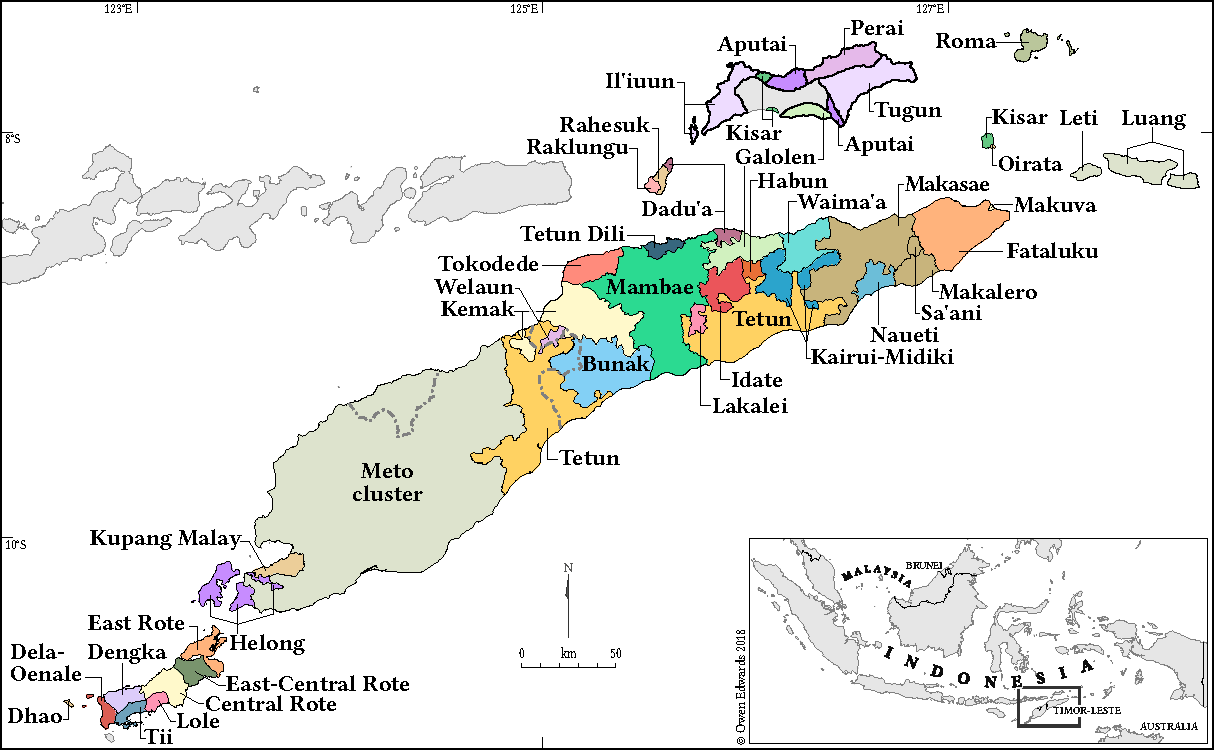
\includegraphics[width=\columnwidth]{TimorLanguages-LinLib.pdf}
\end{figure}

Meto speakers think of their speech as a single language
and call it \it{(uab) metoʔ}, \it{(bahasa) timor}
or occasionally \it{(bahasa) dawan}.
Speakers also recognize more than a dozen named varieties of Meto.
These varieties themselves have named dialects,
with further differences found between different villages and hamlets of a single dialect.
A map of self-identified Meto varieties is given in \frf{fig:SelIdeVarUabMeto}.

\begin{figure}[ht]
	\caption{Self-identified varieties of Meto}\label{fig:SelIdeVarUabMeto}
	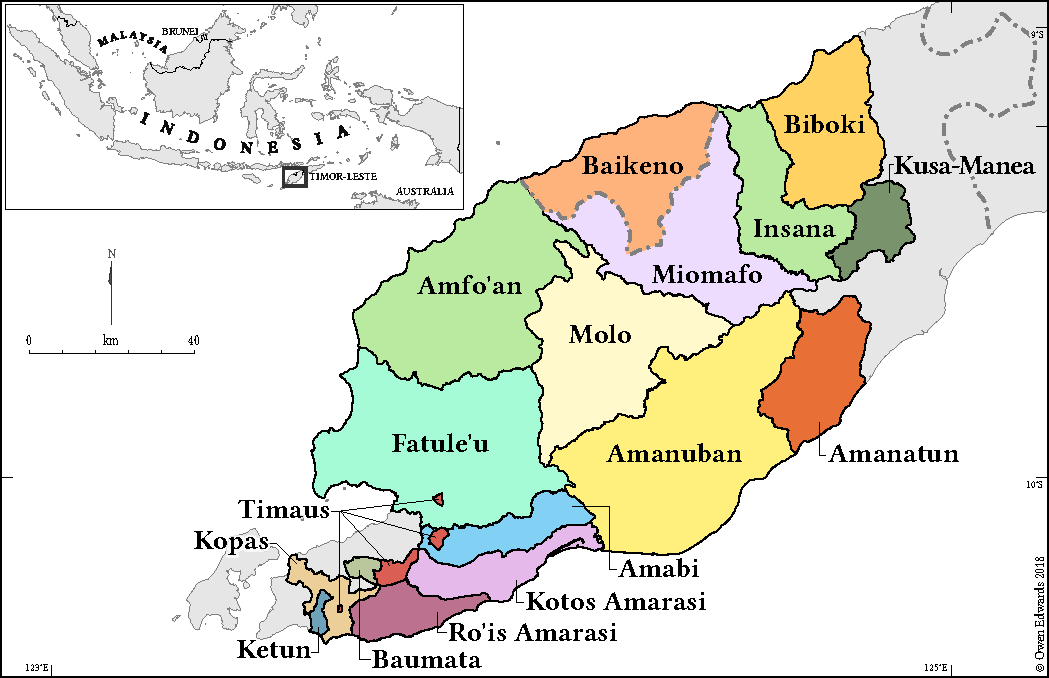
\includegraphics[width=\columnwidth]{Metos-LinLib.pdf}
\end{figure}

The borders of the self-identified varieties of Meto shown in \frf{fig:SelIdeVarUabMeto}
match closely the borders of the pre-colonial political kingdoms of western Timor.\footnote{
		The main exceptions are Kusa-Manea, which was
		part of the Tetun speaking Wehali kingdom,
		as well as Timaus, Baumata, Kopas, and Ketun, which all
		appear to be the result of migrations from more northerly areas.}
The extent to which these boundaries follow linguistic differences is unknown.
In reality, the Meto cluster is a complex language/dialect chain,
and is comparable to more well known cases such as the German chain or the Romance chain.
The nature and extent of variation among Meto varieties has not been fully studied.
Phonological, lexical, semantic, and grammatical diversity is not insignificant
and speakers frequently report difficulty communicating with speakers of other varieties.
As a result, Meto speakers of different varieties often
use a mixture of Meto and Indonesian/Kupang Malay in order to communicate.

\subsection{Affiliation}
Within Austronesian, Meto belongs to the Malayo-Polynesian subgroup
which includes all Austronesian languages outside of Taiwan.
It would further belong to Central Malayo-Polynesian
within Central-Eastern Malayo-Polynesian
\citep{bl81,bl93,bl09b} but the extent
to which these constitute valid
linguistic subgroups is contested \citep{ro95,ad05,dogr08}.

Closer to home, the nearest genealogical relative of Meto is the Rote cluster
spoken on the island of Rote just to the south-west of Timor.
Based on shared sound changes, Rote-Meto can be placed in a Timor-Babar
subgroup which contains the Austronesian languages of Timor and south-west Maluku
(from Babar island to Wetar island), though excluding
Mambae, Tokodede, Welaun, and Kemak which
form a Central Timor subgroup \citep{ed18d,ed19}.

While Meto is demonstrably Austronesian,
it has strong influence from at least one -- probably more --
pre-Austronesian languages of the region \citep{ed16c,ed18b}.
This substrate is reflected at all levels of the language:
lexicon, phonology, morphology, and syntax.

Typologically, Meto fits well in the Melanesian linguistic area with four to five
of the six properties identified by \cite{sc15} as constituting this area.
The only property of linguistic Melanesia which Meto unambiguously lacks
is that of having complex numerals below ten.
Apart from this Meto has genitive-noun order,
absence of velar nasal /ŋ/, noun-numeral order
and possessive classification,
all of which are typical of linguistic Melanesia.

Another property of linguistic Melanesia is verb-negator order.
Regarding this property, most varieties of Meto
for which data is available have double negation
with \ve{ka=} occurring before the verb and \ve{=fa} after the verb.
However, Ro{\Q}is Amarasi has post-verbal \ve{=maeʔ}
while Amfo{\Q}an only has pre-verbal \ve{ka=}.

While Meto fits well within linguistic Melanesia,
it is, based on current understanding,
only a peripheral member of linguistic Wallacea as identified by \cite{sc15}.
\citeauthor{sc15} gives four properties of linguistic
Wallacea: cognates of \su{\#}muku `banana', neuter gender,
semantic alignment, and synchronic metathesis.
Of these, Meto only has synchronic metathesis.

\subsection{Amarasi}\label{sec:Amarasi}
Amarasi is spoken towards the south-west end of the Meto speech area.
One salient feature which sets Amarasi apart from most other Meto
varieties is the liquid /r/ instead of /l/;
most Meto varieties have only a single liquid.\footnote{
		Amabi also has /r/ instead of /l/ as does
		Kusa-Manea, though /l/ occurs in many Tetun loanwords in Kusa-Manea.
		Timaus has both /l/ and /r/ due to a *{\j} > /r/ sound change.}

Amarasi speakers identify three Amarasi dialects: Kotos, Ro{\Q}is, and Tais Nonof.
Current data indicates that Tais Nonof is a label for the speech of
those living along the coast of the Amarasi area,
including those whose speech is most similar to Kotos Amarasi
and those whose speech is most similar to Ro{\Q}is Amarasi.
Amarasi speakers also report that the Amabi variety of Meto
is very similar to their own speech with minor lexical differences.

Differences between Kotos Amarasi and Ro{\Q}is Amarasi
include different functors (grammatical morphemes),
lexicon, phonotactics, as well as having undergone different sound changes.
A number of functors in Ro{\Q}is and Kotos Amarasi
are shown in Table \ref{tab:DifKotRoqFun}
as a sample of the divergence between these two lects.

\begin{table}[h]
	\caption{Different Kotos and Ro{\Q}is functors}\label{tab:DifKotRoqFun}
		\begin{tabular}{lll|lll}
		\lsptoprule
				Kotos 		&Ro{\Q}is 			&gloss		&Kotos 			&Ro{\Q}is 	&gloss	\\ \midrule
				\ve{he}		&\ve{nu}				&{\he}		&\ve{ia}		&\ve{ai}		&{\ia}	\\
				\ve{reʔ}	&\ve{heʔ}				&{\req} 	&\ve{nee}		&\ve{nae}		&{\nee} \\
				\ve{ka={\ldots}=fa}
									&\ve{maeʔ}			&{\kaah}	&\ve{iin}		&\ve{hiin}		&{\iin}	\\
				\ve{on}		&\ve{en}				&{\on}		&\ve{=een}	&\ve{=heen}	&{\een} \\
				\ve{n-bi}	&\ve{n-biʔaak}	&{\bi}		&\ve{nai}		&\ve{neu}		&already \\
				\ve{et}		&\ve{ek/et}			&{\et}		&\ve{u-}		&\ve{ku-}		&{\qu}	\\
				\ve{n-ak}	&\ve{tauʔ/n-ak}	&{\ak}		&\ve{-k}		&\ve{-r}		&\tsc{3pl.gen}\\
				\ve{n-eu}	&\ve{n-uu}			&{\eu}		&\ve{a-{\ldots}-t}&\ve{ka-{\ldots}-t}&\tsc{\at}\\
			\lspbottomrule
		\end{tabular}
\end{table}

In fact, looking only at linguistic structures
and shared sound changes, Kotos Amarasi is more closely
related to other varieties of Meto than it is to Ro{\Q}is Amarasi.
Nonetheless, speakers of Kotos and Ro{\Q}is
self-identify their speech as more similar to one another
than to other Meto varieties.
They frequently interact together
and both share a common history as members of the Amarasi kingdom.
Thus, from a socio-historical perspective,
Kotos and Ro{\Q}is can be considered
``dialects'' of a single language.\footnote{
	Kotos and Ro{\Q}is speakers perceive their speech
	as closer to one another based on salient commonalities
	not found in nearby varieties of Meto.
	Such commonalities include /r/ instead of /l/ and
	lexical items, such as \ve{koʔu}
	`big' instead of \ve{ʔnaek}, or
	\ve{n-kono} `keep going' instead of \ve{n-fini}.}

Data from Kotos Amarasi forms the basis of this book.
I present Ro{\Q}is Amarasi data at various points when it bears on the analysis
of Kotos Amarasi and/or differs in important respects.
My Kotos data comes mostly from the hamlet \emph{(kampung)} Koro{\Q}oto,
in the modern village \emph{(desa)} Nekmese{\Q}.
My Ro{\Q}is data comes from the hamlet
of Suit in the village of Buraen, as well as the hamlets
of Batuna and Ruanrete in the village of Tunbaun.
The locations of these villages within the Amarasi
speech area are shown in \frf{fig:LocNekBurTun}.

\begin{figure}[ht]
	\caption{Locations of Nekmese{\Q}, Buraen, and Tunbaun}\label{fig:LocNekBurTun}
	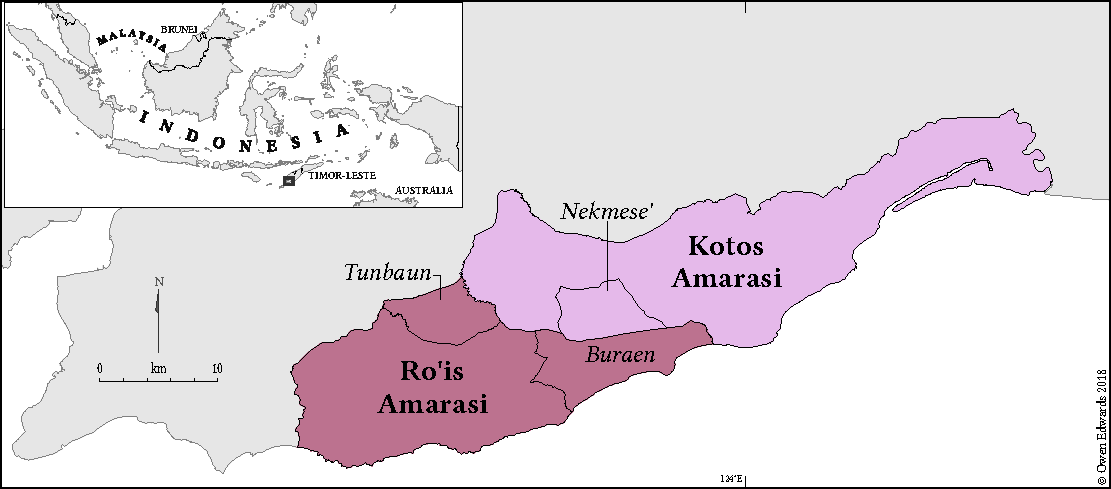
\includegraphics[width=\columnwidth]{Amarasis-LinLib.pdf}
\end{figure}

From 1968--1975 west Timor underwent an administrative restructure
with the creation of the administrative units of districts
(\emph{kecamatan}) and villages (\emph{desa}).
In Amarasi 60 hamlets were amalgamated into 23 villages.
In parts of Amarasi this amalgamation was also accompanied by the 
physical relocation of traditional hamlets in order to allow
for a more efficient development of infrastructure and delivery of services.

Nekmese{\Q} -- data from which forms the core of this work --
was created by the amalgamation of four hamlets:
Koro{\Q}oto, Fo{\Q}asa{\Q}, Tuamese{\Q} and Naet.
These hamlets still exist as \emph{dusun}
(the administrative level below \emph{desa})
and form the basis of the parishes of the dominant
Christian denomination in the village
(the protestant GMIT church\footnote{
		GMIT is an acronym of \emph{Gereja Masehi Injili di Timor};
		for which the official translation is `The Evangelical Protestant Church of Timor'.
		There are four GMIT parishes in Nekmese{\Q}:
		one serving Koro{\Q}oto, one for Fo{\Q}asa{\Q} and Tuamese{\Q}, and two for Naet.})
People also maintain their gardens and fields in the vicinity of the old hamlets.\footnote{
		Inhabitants of Koro{\Q}oto have moved the furthest,
		with \emph{desa} Nekmese{\Q} being located close to the original locations
		of Fo{\Q}asa{\Q} and Tuamese{\Q}.
		The inhabitants of Naet have moved from their original location
		towards Nekmese{\Q}, but Naet remains dislocated from the rest of Nekmese{\Q}.
		The inhabitants of Naet speak the Tais Nonof variety of Amarasi.}

Despite the administrative and physical restructure of 1968--1975,
the traditional hamlets of Nekmese{\Q} are alive and well as distinct social and linguistic units.
A summary of the speech variety which is the focus of this work is given in \qf{ex:SpeVar} below.
Unless explicitly labelled otherwise,
all data is Kotos Amarasi from the hamlet of Koro{\Q}oto.

\begin{exe}
	\ex{
		\begin{xlist}
			\ex{Language: \emph{Meto}}
			\ex{Variety: \emph{Amarasi}}
			\ex{Dialect: \emph{Kotos}}
			\ex{Hamlet: \emph{Koro{\Q}oto}}
		\end{xlist}
	}\label{ex:SpeVar}
\end{exe}

\section{Previous work}\label{sec:PreWor}
The earliest description of Meto known to me is \cite{mu57},
which contains a wordlist in what is probably a variety of Molo.
After this, the next earliest work is \cite{kl94}
which contain what appears to be an Amanuban wordlist,
though forms from other varieties are also given.

There are also works by the Dutch linguist
J. C. G. Jonker which contain data on Meto.
This includes \cite[270f]{jo04} which is a one page
glossed Amfo{\Q}an text with notes.
\cite{jo06} discusses word-final consonants in a number of
Austronesian languages including Meto.
The Meto data in \cite{jo06} is mostly Amfo{\Q}an, though data on
other varieties, including Amarasi, is also given.
Much of \citeauthor{jo06}'s Meto data also
occurs in etymological notes in \cite{jo08};
an 805-page dictionary of the Termanu variety of the Rote cluster.

\cite{ca44} provides a wordlist in Meto ``from Dutch sources''.
This appears to be based on Jonker's data
and \cite{jo06} is the source for
the discussion of final consonants in \cite[29]{ca44c}.

The first in depth treatment of Meto is that
of the Dutch missionary Pieter Middelkoop.
\citeauthor{mi39} published a collection of Amarasi texts \citep{mi39}
which had been previously collected by Jonker, a collection
of funeral chants \citep{mi49}, and a sketch grammar of Molo \citep{mi50}.
The other work by Middelkoop is an unpublished 673-page draft dictionary of Molo,
which was still in preparation before his death \citep{mi72}.\footnote{
		Thanks goes to James Fox for giving me his copy of \cite{mi72}.}
\citeauthor{mi39}'s materials on Meto contain much valuable data.
However, the transcription employed by \citeauthor{mi39} is not phonemic
and certain contrasts are under-represented.
%In order to assist future researchers I give
%here the most common transcriptional issues one encounters
%when working with \citeauthor{mi39}'s material.
%
%\begin{itemize}
	%\item The glottal stop /ʔ/ is often written as <{\Q}> between two vowels.
				%Word initially, before consonants, and word finally it is not usually written.
	%\item In \cite{mi39,mi50} the grave accent sometimes marks double vowels,
				%and sometimes phonetic vowel quality and/or stress.
				%In particular the mid-low allophone [ɛ] of /e/ is usually written \it{<è>}
	%\item A final apostrophe in \cite{mi72} marks a double vowel.
	%\item Both /ao/ and /au/ are transcribed \it{<au>}.
	%\item Prefixes consisting of a single consonant are often written
				%with a previous vowel-final word.
	%\item The final vowel of the pronouns \ve{ina} `{\iin}', \ve{sina} `{\siin}', \ve{hita} `{\hiit}'
				%is usually written with a following inflected verb.
%\end{itemize}

There are also a number of papers on Meto by Hein Steinhauer,
who worked on the Nilulat dialect of Miomafo.
This includes a description of verb morphology \citep{st93}
and a series of papers which provide an initial
description of the form of metathesis within the noun phrase
\citep{st96,st96b,st08}.

Other works which I have been able to access
on Meto include a Masters Thesis on Miomafo \citep{ta88},
a grammar produced by the Indonesian Pusat Bahasa \citep{ta89},\footnote{
		Thanks goes to Patrick McConvell for providing me
		with his copies of \citet{ta88} and \citet{ta89}.}
a description of quantification in Amanuban \citep{mebe14},
an Optimality Theory account of the segmental phonology of Miomafo \citep{is13},
a description of consonant insertion in Nai{\Q}bais Amfo{\Q}an \citep{cu18},
and a discussion of serial verb constructions in Amarasi
as being one source of similar constructions in Kupang Malay \citep{jagr11}.

\section{Data for this work}\label{sec:Meth}
The core of the Amarasi data on which this work is based
is a corpus of recorded texts totalling nearly nineteen hours
of which about five hours has been processed.
This includes a little more than three hours of
transcribed, translated, and glossed Kotos texts,
as well as just over two hours of transcribed and translated Ro{\Q}is texts.
These texts are of a variety of genres and include narratives, folk-tales,
conversations, and traditional poetry.

An index of the texts which comprise this corpus is given in Appendix
% \ref{app:TexInd}.
D.
These texts are archived with the
Pacific And Regional Archive for Digital Sources in Endangered Cultures (PARADISEC)
and nearly all are freely downloadable.

My Kotos texts were collected in three
field trips totalling seven months I made
in 2013, 2014, and 2016 over the course of my PhD work.
During these field trips I was hosted in Timor by
Heronimus Bani (Roni), a native speaker of Amarasi, in the village of Nekmese{\Q}.
These texts were recorded either by me or by Roni
and then transcribed and translated by native speakers of Amarasi, either Roni or Yedida Ora (Oma).
I then checked the initial transcriptions against the recording and glossed the text in Toolbox.
All my Kotos Amarasi texts can be accessed
from \url{http://catalog.paradisec.org.au/collections/OE1}.

During 2012 I was a participant in a two week
language documentation workshop held in Kupang:
\emph{Preserving Knowledge through Recording and Writing Local Languages}.
During this workshop a number of additional Kotos Amarasi
texts were recorded and transcribed by Oma.

My Ro{\Q}is texts were collected during a
field trip at the end of 2018
while undertaking an Australia Awards Endeavour Fellowship.
During this trip I spent one week in Buraen
with Toni Buraen and his family, followed by
two weeks in Tunbaun with Melianus Obhetan and his family.
I transcribed my Ro{\Q}is Amarasi texts
and then checked them with native speakers.
My Ro{\Q}is Amarasi texts can be downloaded from
\url{http://catalog.paradisec.org.au/collections/OE2}.

In addition to this text corpus, I also conducted a number of
elicitation sessions with Roni in 2016.
This elicitation involved working through recorded texts with Roni
and manipulating individual parts of sentences for grammaticality judgements.
When a manipulated sentence was accepted as grammatical,
I would then have Roni say it back to me.
This often resulted in him rejecting a sentence he had originally accepted.
Elicitation was also carried out with Oma on a number of occasions.

This data is supplemented by a translation
of the New Testament and Genesis into Kotos Amarasi: \citet{UBB15}.\footnote{
		This translation can be accessed online at \url{www.e-alkitab.org}
		or downloaded for free on Android devices from Google Playstore (search: Amarasi Bible).}
This translation was carried out by native Amarasi speakers
and is completely natural and idiomatic Amarasi as evidenced
by the fact that it is full of grammatical constructions that differ
from both Indonesian and Kupang Malay (used as front translation).
Before publication this translation was checked with at least three different
groups of native speakers comprising three or more speakers in each group
(representing a good cross section of age, gender, and educational levels) for clarity and naturalness.
The material was tested and further refined with each successive group,
then followed by a smoothing read-through looking at naturalness and flow before publishing.

Data from this translation is presented
when it contains good, clear exemplars of rare constructions.
However, no part of my analysis rests
solely on data found only in the Amarasi Bible translation.
See \cite{hehawi11} and \citet[2]{dryer13} for discussion of
the use of Bible translations as sources of linguistic data.

A final source of Kotos Amarasi data is a series
of primary school readers translated from Kupang Malay
into Amarasi by Yedida Ora \citep{or16,or16b,or16c}.
These readers have also been checked and edited for naturalness and fluency.

In addition to all this Amarasi data, I also have also
collected data on the following varieties of Meto,
some of which appears at various points in this book:
Timaus (half an hour of transcribed, translated, and glossed texts,
as well as 1 hour 15 minutes untranscribed texts, lexicon of 685 headwords),
Kusa-Manea (four hours of untranscribed texts, lexicon of 488 headwords),
Amanuban (22 untranscribed texts, 8 wordlists),
Ketun (3 untranscribed texts, 3 wordlists),
Kopas (3 untranscribed texts, 5 wordlists),
Fatule{\Q}u (2 wordlists), and
Amfo{\Q}an (1 wordlist).
I also have Baikeno data collected during
the 2012 Kupang language documentation workshop,
as well as data collected and provided by Charles Grimes.
Unless otherwise cited, all Meto data in this book comes
from these sources.

\section{Presentation of data and notational conventions}\label{sec:PreDat}
Data from Amarasi, or another variety of Meto,
is transcribed phonemically and presented in italic font.\footnote{
		There are only three non-phonemic aspects of my transcription.
		Firstly, foreign proper names are transcribed orthographically
		when they contain non-native phonemes the IPA representation
		of which is not identical to their orthographic, e.g. \ve{Lince} [li{\ny\tS}e].
		Secondly, /ɡw/ is transcribed \it{<g>} before rounded vowels (\srf{sec:VoiObs}).
		Thirdly, /n/ {\ra} [ŋ] is transcribed \it{<ng>} when it occurs before /ɡw/
		without an intervening morpheme break.
		These last two non-phonemic conventions
		can be seen in the word for `teacher',
		which according to my analysis has the form /tunɡwuru/,
		but is transcribed as \ve{tuŋguru}.}
Example sentences are given with up to two gloss lines.
A typical example is given in \qf{ex:120715-4, 0.55 ch:Intr} below.

\begin{exe}
	\ex{\glll	\sf{ahir{\ny}a} ahh, n-aim naan baar\j=esa =m na-maikaʔ n--\\
						\sf{ahir{\ny}a} {} n-ami naan bare=esa =ma na-maikaʔ {}\\
						in.the.end {} 3-look.for{\M} {\naan} place{\Mv}={\es} =and {\na}-settle {}\\
			\glt	`In the end, he looked there for a place and settled.'
						\txrf{120715-4, 0.55} {\emb{120715-4-00-55.mp3}{\spk{}}{\apl}}}\label{ex:120715-4, 0.55 ch:Intr}
\end{exe}

The first line is the phonemic transcription with morpheme breaks indicated.
Affixes are separated by the hyphen -.
Enclitics are separated from their host by the equals sign =.
Vowel initial enclitics which induce morphophonemic processes on their
host (Chapter \ref{ch:PhoMet}), are attached directly to the host,
while other enclitics are offset.
An example of each kind of enclitic can be seen in \qf{ex:120715-4, 0.55 ch:Intr}
with vowel initial \ve{=esa} `one' and consonant initial \ve{=m} `and'.

Word-initial epenthetic /a/ is separated by the vertical line |.
The underscore {\gap} is used to separate two parts of a phrase with
a non-compositional meaning or phrases where
one element does not occur independently.
An example of epenthesis occurs in \ve{a|n-kobub}
`piled up' in \qf{ex:120715-4, 0.05 ch:Int} below,
and an example of a non-compositional phrase is
\ve{paha{\gap}ʔpinan} `country{\gap}below' = `world'
in \qf{ex:120715-4, 0.05 ch:Int}.

Instances of Indonesian/Kupang Malay code-switching or unassimilated loans 
are transcribed in a sans-serif typeface.
Thus, in example \qf{ex:120715-4, 0.55 ch:Intr} the word
\ve{\sf{ahir{\ny}a}} `in the end' is from Kupang Malay \it{ahirnya}.
Phonetic strings which are pauses are indicated by a final \it{<hh>} and are usually unglossed.
In example \qf{ex:120715-4, 0.55 ch:Intr} \ve{ahh} is a pause
with the phonetic quality approximating [aːː],
similarly \ve{nehh} is a pause which sounds like [nɛːː].
False starts are not glossed and indicated by a final en-dash --.
One example is the final \ve{n--} in example \qf{ex:120715-4, 0.55 ch:Intr} above.
Commas indicate pauses and/or intonation breaks
and full stops represent the end of an intonation unit.
Capital letters are only used for proper names.

The second line gives the underlying form
of morphemes before processes of metathesis, consonant insertion, and vowel assimilation occur.
It also gives the underlying forms of enclitics which have multiple forms (\srf{sec:SenEnc}).
The third line gives the morpheme by morpheme gloss.
When a morpheme is ambiguous between several values,
these values are separated by a slash /. An example
is the verbal agreement prefix \ve{m-} `{\m}' which
agrees with first person exclusive,
second person singular, and second person plural.
Glosses mostly follow the Leipzig Glossing Rules
with a full list of glosses used in this book,
including non-standard glosses, given beginning on \prf{ch:Abb}.

\begin{table}[ht]
	\caption{Glosses for U-forms and M-forms}\label{tab:GloUfoMfo}
		\begin{tabular}{ll}
			\lsptoprule
						Gloss & Use \\ \midrule
				\tsc{u}		& U\=/form \\
				%\tsc{u\shiftleft{1.3pt}{\scalebox{2.0}{ͨ}}}		& 1. U\=/form of consonant-final stem\\
				\tsc{u\raisebox{-4pt}{\scalebox{1.75}{ͨ}}}		& 1. U\=/form of consonant-final stem\\
									& 2. U\=/form before consonant cluster\\
				\tsc{m}		& M\=/form\\
				\tsc{m\shiftleft{0.8pt}{̿}}		& M\=/form before vowel-initial enclitic \\
				\tsc{m\shiftleft{0.25pt}{\raisebox{-4pt}{\scalebox{1.75}{ͨ}}}}		& M\=/form before consonant cluster\\
			\lspbottomrule
		\end{tabular}
\end{table}

Glosses indicating U\=/forms and M\=/forms
are usually only given when potentially relevant to the discussion at hand.
Glosses for U\=/forms and M\=/forms in different phonotactic environments are given in \trf{tab:GloUfoMfo},
with a number of examples given in \qf{ex:120715-4, 0.05 ch:Int}--\qf{130821-1, 6.20} below.
See Chapter \ref{ch:StrMetAma} for more discussion of the distribution
of each of these forms.
Glosses for U\=/forms or M\=/forms are not given when a form
does not distinguish between them.

\begin{exe}
	\ex{\glll	neno naa paha{\gap}ʔpina-n ia, a|n-kobub on bare meseʔ\\
						neno naa paha{\gap}ʔpina-n ia	{\a}n-kobub on bare meseʔ\\
						day{\tbrU} {\naa} land{\gap}below{\tbrU}-{\N} {\ia} {\a\n}-pile{\tbrUc} {\on} place{\tbrU} one\\
			\glt	`In those days the world was piled up in one place.'
						\txrf{120715-4, 0.05} {\emb{120715-4-00-05.mp3}{\spk{}}{\apl}}}\label{ex:120715-4, 0.05 ch:Int}
	\ex{\glll	uma ʔ-tee =ma, ʔ-aiti bruuk.	\\
						uma ʔ-tea =ma ʔ-aiti bruuk \\
						{\uma\tbrUc} \q-arrive =and \q-pick.up{\tbrUc} pants{\U}	\\
			\glt	`I arrived (home) and picked up some pants.'
						\txrf{130825-6, 10.05} {\emb{130825-6-10-05.mp3}{\spk{}}{\apl}}}\label{130825-6, 10.05 ch:Int}
	\ex{\glll	hii m-euk siis\j=ii =m	\\
						hii m-eku sisi=ii =ma\\
						{\hii} \m-eat{\tbrM} meat{\tbrMv}={\ii} =and	\\
			\glt	`You ate the meat and' \txrf{120923-1, 6.01} {\emb{120923-1-06-01.mp3}{\spk{}}{\apl}}}\label{120923-1, 6.01}
	\ex{\glll	afi{\gap}naa au ʔ-tae iin sura srainʔ=ii =t	\\
						afi{\gap}naa au ʔ-tae ini surat sraniʔ=ii =te	\\
						yesterday {\au} ʔ-look.down {\iin} paper{\tbrMc} baptism{\tbrMv}={\ii} ={\te}\\
			\glt	`Yesterday when I looked at her baptismal certificate,'
						\txrf{130821-1, 6.20} {\emb{130821-1-06-20.mp3}{\spk{}}{\apl}}}\label{130821-1, 6.20}
\end{exe}

Gloss lines are followed by a free translation into English.
Words not present in the Amarasi example
but supplied in the free translation to increase
its naturalness are enclosed in brackets ().
Important para-linguistic information such as gestures
are described in square brackets [] in the free translation.
Occasionally a literal translation of part or all of the Amarasi example is given.
Literal translations are enclosed in brackets and preceded by the abbreviation `\emph{lit.}'.

The numeric code to the right of the free translation
is a reference to which text the example comes from.
These codes follow the format \emph{yy-mm-dd-no., time in text}.
Thus, the code {\ttfamily 120715-4, 0.55} in example \qf{ex:120715-4, 0.55 ch:Intr} above
indicates that this example begins at about 55 seconds
into the fourth recording made on the 15/07/2012.

Examples with the speaker icon \spk{}
have an accompanying sound file.
These
sound files can be downloaded from TROLLing (The Tromsø Repository of Lan-
guage and Linguistics) at \url{https://doi.org/10.18710/IORWF6}  \citep{ed20}. These
sound files are organised in the repository according to the chapter in which they
occur with additional information on their specific location, such as example or
table number, embedded in the file name. See the ReadMe in the TROLLing repos-
itory for a complete explanation.


In addition to examples from my text collection,
three other kinds of examples occur.
Firstly, data which was encountered during the course
of my fieldwork but not recorded is indicated as \emph{observation}
usually with the date and page reference to my notebook; e.g. {\ttfamily observation 09/10/14, p.113}.
Secondly, data which were collected during elicitation are marked as \emph{elicit.}
with the date and page reference to my notebook; e.g. {\ttfamily elicit. 15/03/2016 p.47}
Finally, data from the Amarasi Bible translation are referenced
by book, chapter, and verse, e.g. {\ttfamily John 3:16}.

When longer examples from a single text are given,
a short description usually precedes the text
(followed by the unique code cross referencing the text).
The data following this title is then labelled alphabetically.
An example is given in \qf{ex:120715-4, 0.43-0.45 ch:Intr} below.
When an example involves more than one speaker,
different speakers are indicated with Greek letters.

\largerpage
\begin{exe}
	\ex{How Moo{\Q}-hitu made the world:
				\txrf{120715-4} {\emb{120715-4-00-43-00-45.mp3}{\spk{}}{\apl}}}\label{ex:120715-4, 0.43-0.45 ch:Intr}
	\begin{xlist}
		\ex{\glll	n-bi{\tl}bi oo\j=ee naan-n=ee {onai =te},\\
							n-bi{\tl}bi oe=ee nana-n=ee {onai =te}\\
							\n-{\prd}{\bi} water={\ee} inside-{\N=\ee} and.then\\
				\glt	`Having been in the water for a while,' \txrf{0.43}}\label{ex:120715-4, 0.43 ch:Intr}
\clearpage
		\ex{\glll	a|n-moʔe =ma n-poo\j=ena n-bi metoʔ.\\
							{\a}n-moʔe =ma n-poi=ena n-bi metoʔ\\
							{\a\n}-make =and \n-exit={\een} {\n}-{\bi} dry\\
				\glt	\lh{a|}`(he) made and went out onto dry land.' \txrf{0.45}}\label{ex:120715-4, 0.45 ch:Intr}
	\end{xlist}
\end{exe}

When data on languages other than Amarasi or Meto is cited,
such data is transcribed in italics phonemically according to IPA conventions.\footnote{
		For the sake of complete clarity, the palatal glide /j/
		is always transcribed \it{<j>} while the 
		palatal affricate /\j/ is always transcribed \it{<\j>}.}
Data from languages with a widely used standard
orthography are usually transcribed orthographically followed
by a phonemic IPA transcription, an example is English \it{mouse} /maʊs/.

\section{Goals and the use of theory}\label{sec:GoaUseThe}
The main goal of this book is to present an accurate
description of the forms and functions of metathesis in Amarasi
(chapters \ref{ch:StrMetAma}--\ref{ch:DisMet}).
A secondary goal is to propose a clear analysis of the data.
A third goal to situate the Amarasi data within
its typological, geographical, and cultural context
(Chapters \ref{ch:SynchMet} and \ref{ch:ConCon})

Notably, it is \emph{not} the main goal of this book to
present the Amarasi data as an argument in
favour of any particular theoretical model.
While I make frequent use of representations and
tools from different theoretical models,
I do so mainly to illustrate clearly
aspects of the Amarasi data in a helpful way
and as explicit strategy to summarise certain generalisations.

Thus, in Chapters \ref{ch:StrMetAma} and \ref{ch:PhoMet}
I make use of Autosegmental theory as it helpfully
illustrates the processes which occur in the derivation of M\=/forms from U\=/forms.
Similarly, in describing M\=/forms before consonant clusters
\srf{sec:CCIniMod} I make use of Optimality Theory
as the tableaux of this theory illustrate well the large
number of potential outputs a particular string could generate.
Likewise, in Chapter \ref{ch:SynMet} I make use of X-bar theory to analyse
the role of metathesis within the syntax.

In general, different theoretical models
and the analyses these entail are deployed in this book
in an expedient manner according to what seems most
illuminating for the Amarasi data.
The primary use of theory is to present a clear and simple
analysis of Amarasi metathesis,
not a theoretically consistent analysis.
Thus, the observant reader will note, for instance,
that in my account of phonologically conditioned metathesis
in Chapter \ref{ch:PhoMet} I make frequent use of
constraints developed within Optimality Theory
without ever presenting an Optimality Theory tableau.
While I find some Optimality Theory constraints helpful
in understanding the data, an actual account embedded within Optimality Theory
clouds rather than illuminates the description.\footnote{
		This is not to say that Optimality Theory is wrong,
		or that it cannot or should not be used to analyse Amarasi metathesis.
		Instead, I merely do not find a full Optimality Theory account
		of this aspect of Amarasi metathesis a helpful aid.}

The main exception to this approach is in the analysis
of the structure of metathesis in Chapter \ref{ch:StrMetAma}.
In this chapter I explicitly formulate an analysis
using an autosegmental model of phonology \citep{go76}
and a rule-based model of process morphology \citep{ma74,an92}.
I do this because these models allow me to propose a
unified analysis of the form of Amarasi metathesis.

However, my primary commitment is not to any particular theory,
or any particular analysis, but to the Amarasi data itself.
I would welcome criticism of the analyses
proposed in this book so long as any alternate analyses
remain faithful to the primary data upon which any analysis must be based.
Similarly, I would welcome any dialogue with this book
which attempts to provide a unified theoretical account of all of the data.
\section{Terminology}\label{sec:Ter}
In this section I give definitions of potentially ambiguous linguistic terminology.
The definitions given here should be taken only as a practical guide
to understand how terms are used in this book
and should \emph{not} be taken as strong claims
about the theoretical status of any of the elements defined.

As used in this book, a \emph{word} is the minimal meaningful
phonological string which can occur in isolation.\footnote{
		Two typical environments in which words occur in isolation are
		in response to a question or in collection of a wordlist.
		Likewise, pauses are not usually allowed in the middle of a word.
		If such a pause occurs, the speaker usually repeats the entire word from the beginning.}
A \emph{morpheme} is ``an indivisible stretch of phonetic (or phonological)
material with a unitary meaning'' \citep[49]{an92}.\footnote{
		In many morphological theories the morpheme does not play a central role,
		including \cite{ma74,an92} and \cite{st01}.
		While I am extremely sympathetic to such theories,
		the morpheme is still a useful analytic tool for much of the Amarasi data.}
A \emph{root} is an underlying single morpheme without any affixes attached.

We can furthermore distinguish between \emph{bound} and \emph{free morphemes}.
A free morpheme is a root which can occur as a word without any other morphemes attached.
A typical example is \ve{kaut} `papaya'.
A bound morpheme is a root which cannot occur as a word.
Instead a bound morpheme must surface attached to another morpheme.
A \emph{clitic} is a morpheme which is phonologically bound
to a clitic host, but has a separates syntactic status to the host.
A typical example is the determiner \ve{=ee}, which marks definiteness.
While this determiner must occur attached to a host (e.g. \ve{kaut=ee} `the papaya')
which is the head of a noun phrase, the enclitic itself 
is the head of a separate determiner phrase (\srf{sec:DetPhr}).
My definitions of all these terms when applied to Amarasi or Meto data
are summarised in \qf{ex:TerDef} below, with a number of examples also given.

\begin{exe}
	\ex{Terminological definitions \txrf{}}\label{ex:TerDef}
	\begin{xlist}
		\ex{Morpheme = indivisible phonetic stretch with unitary meaning}
			\sn{\ve{n-} `third person verbal agreement', \ve{kobub} `pile up', \ve{kaut} `papaya', \ve{=ee} `{\ee}, third person determiner'}
		\ex{Word = minimal phonological string which can occur in isolation}
			\sn{\ve{n-kobub} `piles up', \ve{kaut} `papaya', \ve{kaut=ee} `the papaya'}
		\ex{Bound morpheme = morpheme which cannot occur as an independent word}
			\sn{\ve{n-} `third person verbal agreement', \ve{=ee} `{\ee}'}
		\ex{Root = underlying single morpheme}
			\sn{\ve{{\rt}n-} `third person verbal agreement', \ve{{\rt}kobub} `pile up', \ve{kaut} `papaya', \ve{{\rt}=ee} {\ee}}
		\ex{Free morpheme = morpheme which is an eligible word}
			\sn{\ve{kaut} `papaya', \ve{teun} `three'}
		\ex{Affix = bound morpheme with no separate syntactic status to its host}
			\sn{\ve{n-} `third person verbal agreement', \ve{-m} {\mg} `first person exclusive or second person genitive'}
		\ex{Clitic = bound morpheme with different syntactic status to its host}
			\sn{\ve{=ee} `{\ee}', \ve{=ma} `and', \ve{=kau} `{\kau}'}
		\ex{Stem = a word or root to which a bound morpheme attaches}
			\sn{\ve{n-\tbr{kobub}} `piles up', \ve{\tbr{kaut}=ee} `the papaya'}
		\ex{Citation Form = usual form of a word given in wordlist style elicitation}
	\end{xlist}
\end{exe}

I also make a distinction between two kinds of words and roots,
\emph{functors} and \emph{lexical words/roots} \citep[85ff]{zo78,gr91}.
Functors are morphemes which have grammatical uses,
such as relativisers, demonstratives, topic markers, and pronominals,
while lexical words/roots typically refer to events, states, properties, and things.

